\documentclass{beamer}

\DeclareOptionBeamer{slidesperpage}{2}

%\usefonttheme[onlymath]{serif}
\mode<presentation>
{
  \usetheme{default}
  % or ...

  \setbeamersize{text margin left=1em,text margin right=1em}
  \setbeamercovered{invisible}
  \setbeamertemplate{headline}
  {
  \begin{beamercolorbox}[wd=\paperwidth,ht=0ex,dp=0ex,right]{date in head/foot}%
    \usebeamerfont{date in head/foot}
    \vspace{-3em}Course Overview\hspace*{2ex} 
  \end{beamercolorbox}
  }
  \setbeamertemplate{footline}
  {
  \begin{beamercolorbox}[wd=\paperwidth,ht=2.5ex,dp=1ex,left]{date in head/foot}%
    \usebeamerfont{date in head/foot}
    \hspace*{2ex}CS 422
    \hspace{\stretch{85}}
    Hal Daum\'e III (UMD)
    \hspace{\stretch{100}}
    \makebox[0in][b]{\insertframenumber{} / \inserttotalframenumber}\hspace*{2ex}
  \end{beamercolorbox}
%  \begin{beamercolorbox}[wd=\paperwidth,ht=2.25ex,dp=1ex,right]{date in head/foot}%
%    \usebeamerfont{date in head/foot}
%    \insertframenumber{} / \inserttotalframenumber\hspace*{2ex} 
%  \end{beamercolorbox}
  }
  % or whatever (possibly just delete it)
}


%\newcommand{\ddx}{\frac \partial {\partial x}}

\usepackage[english]{babel}
% or whatever

\usepackage[latin1]{inputenc}
% or whatever

\usepackage{graphics}
\usepackage{times}
\usepackage{xcolor}
\usepackage[T1]{fontenc}

\usepackage{natbib}
\usepackage{haldefs}
\usepackage{notes-slides}
\bibliographystyle{plainnat}
\bibpunct{[}{]}{,}{a}{,}{,}

% Or whatever. Note that the encoding and the font should match. If T1
% does not look nice, try deleting the line with the fontenc.

\definecolor{DarkGreen}   {rgb}{0,0.5,0}
\definecolor{DarkBlue}    {rgb}{0,0.0,0.5}
\definecolor{LightGray}   {rgb}{0.8,0.8,0.8}


\newcommand{\vsp}{\vspace{1em}}
\newcommand{\blue}[1]{{\color{blue}#1}}
\newcommand{\dblue}[1]{{\color{DarkBlue}#1}}
\newcommand{\green}[1]{{\color{DarkGreen}#1}}
\newcommand{\black}[1]{{\color{black}#1}}
\newcommand{\red}[1]{{\color{red}#1}}

\usecolortheme{default}   % default, albatross, crane, dove, fly, seagull
\setbeamercolor{frametitle}{fg=DarkBlue,bg=LightGray}
\beamertemplatenavigationsymbolsempty

\title[Course Overview] % (optional, use only with long paper titles)
{Course overview and general classes of problems}


\author{Hal Daum\'e III} % (optional, use only with lots of authors)

\date% (optional)
{CS 422: Machine Learning\\\vspace{2em}23 January 2013}

\subject{Talks}
% If you wish to uncover everything in a step-wise fashion, uncomment
% the following command: 

%\beamerdefaultoverlayspecification{<+->}


\begin{document}


\begin{frame}
\frametitle{}
\vsp

~

~


~

~

{\Huge CMSC 422: Machine Learning}

~

~

{\Large Hal Daum\'e III}

~

~


~

~

{\Large 01 Sep 2015}
\end{frame}

\begin{frame}
\frametitle{Course Background}

{\bf What is this course about?}
\bei
\i Finding (and exploiting) patterns in data
\i Replacing ``human writing code'' with ``human supplying data''
\bei
\i[$\Rightarrow$] System figures out what the person wants based on examples
\i[$\Rightarrow$] Need to abstract from ``training'' examples to ``test'' examples
\i[$\Rightarrow$] Most central issue in ML: \emph{generalization}
\eni
\eni

\vsp
\onslide<2>{
{\bf Why is machine learning so cool?}
\bei
\i Broad applicability
\bei
\i Finance, robotics, vision, machine translation, medicine, etc.
\eni
\i Close connection between theory and practice
\i Open field, lots of room for new work
\i \url{http://www.computerworld.com/action/article.do?command=viewArticleBasic&articleId=9026623}
\eni
}
\end{frame}



\begin{frame}
\frametitle{Course Goals}

By the end of the semester, you should be able to:
\bei
\i Look at a problem and identify if ML is an appropriate solution
\i If so, identify what types of algorithms might be applicable
\i Apply those algorithms
\i Conquer the world
\eni

\vsp
In order to get there, you will need to:
\bei
\i Do a lot of math (calculus, linear algebra, probability)
\i Do a fair amount of programming
\i Work hard (this is a 3-credit class)
\eni

\end{frame}


\begin{frame}
\frametitle{Student comments on this course}

\begin{large}
\bei
\i<1-> The field of machine learning seems too wide for any one-semester long course to completely cover everything
\i<2-> This course shouldn't be CS 422, it should be MATH 422!
\i<3-> All in all, great class, and clear interest in the needs of the students
\i<4-> $[$The professor$]$ needs to learn how to write proper exams
\i<5-> \dots and so on \dots
\eni

\vsp
\onslide<6->{
I try to take your comments seriously!

~~~~~~~~\red{(but some things won't change\dots)}
}
\end{large}

\end{frame}


\begin{frame}
\frametitle{Topics Covered}

\bei
\i Supervised learning: \blue{learning with a teacher}
\i Unsupervised learning: \blue{learning without a teacher}
\i Complex settings: \blue{learning in a complicated world}
\bei
\i<2-> Time-series models
\i<2-> Structured prediction
\i<2-> Semi-supervised learning
\i<2-> Large-scale learning
\eni

\vsp
\i<3-> \red{\Large Not a zoo tour!}
\i<3-> \red{\Large Not an introduction to tools!}
\i<4-> \green{\Large You will learn how these techniques work\\and how to implement them.}
\eni
\end{frame}



\begin{frame}
\frametitle{Syllabus}
\vsp
{\Huge On Piazza, linked from \url{http://hal3.name/}}
\end{frame}

\begin{frame}
\frametitle{On Reading and Responsibilities\dots}

\blue{\Huge Reading: I expect you to do it!}

{\Large (but most are $\leq 12$ pages, all are $\leq 20$)}

Online book draft (missing some figures) linked off the web page.  (Extra
credit for new/unique bugs submitted or \emph{fixed} on GitHub!)

\vsp
\vsp
\onslide<2->{
\Large
Class time is for:
\bei
\i Discussing questions from the reading
\bei
\i There are questions in the margins: be prepared to answer them
\eni
\i Discussing homework assignments / labs
\bei
\i On each homework you must answer a ``what didn't you understand'' question
\eni
\i Me providing an insider's view
\eni
}

\end{frame}


\begin{frame}
\frametitle{Things \red{you} need to do \red{now!}}

{\bf Complete Homework 00}
\bei
\i Due 08 Sep (that's \red{next Tuesday!}, by 8:00a)
\i Submit using \blue{handin}
\eni

\vspace{2em}
{\bf Complete the first reading}
\bei
\i See syllabus
\i Due by class Thursday (I mean it!)
\eni

\vspace{2em}
{\bf Sign up to get mails}
\bei
\i Subscribe to the Piazza group.
\i But be sure to actually read it!
\eni

\vspace{2em}
{\bf Read the Piazza course description information!}

\end{frame}


\begin{frame}
\begin{center}
\blue{\huge Now, on to some \black{real} content\dots}
\end{center}
\hspace{20em}(but first, questions?)
\bei
\i<2-> Training/testing
\eni
\end{frame}



\begin{frame}
\frametitle{Classification}

\bei

\i How would you write a program to distinguish a \green{picture} of
\red{me} from a picture of \blue{someone else}?

\bei
\i<2->[$\Rightarrow$] Provide examples pictures of \red{me} and
pictures of \blue{other people} and let a \emph{classifier} learn to
distinguish the two.
\eni

\i How would you write a program to determine whether a
\green{sentence} is \red{grammatical} or \blue{not}?

\bei
\i<3->[$\Rightarrow$] Provide examples of \red{grammatical} and
\emph{ungrammatical} sentences and let a \emph{classifier} learn to
distinguish the two.
\eni

\i How would you write a program to distinguish \red{cancerous}
\green{cells} from \blue{normal} \green{cells}?

\bei
\i<4->[$\Rightarrow$] Provide examples of \red{cancerous} and
\emph{normal} cells and let a \emph{classifier} learn to distinguish
the two.
\eni
\eni
\end{frame}


\begin{frame}
\frametitle{Data (``weather'' prediction)}

{\bf Example dataset:}
\begin{center}
\begin{tabular}{c|ccc}
{\bf \blue{Class}} & {\bf Outlook} & {\bf Temperature} & {\bf Windy?}\\
\hline
\blue{Play}    & Sunny    & Low  & Yes \\
\blue{No play} & Sunny    & High & Yes \\
\blue{No play} & Sunny    & High & No  \\
\blue{Play}    & Overcast & Low  & Yes \\
\blue{Play}    & Overcast & High & No  \\
\blue{Play}    & Overcast & Low  & No  \\
\blue{No play} & Rainy    & Low  & Yes \\
\blue{Play}    & Rainy    & Low  & No  
\end{tabular}
\end{center}

\only<2-7>{
{\bf Three principle components:}
\bee
\i Class label \onslide<3->{(aka \blue{``label''}, denoted $y$)}
\i Features \onslide<4->{(aka \blue{``attributes''})}
\i Feature values \onslide<5->{(aka \blue{``attribute values''}, denoted $x$)}
\onslide<6->{
\bee
\i[$\Rightarrow$] Features can be \blue{binary}, \blue{nomial} or \blue{continuous}
\ene}
\ene
\onslide<7->{\bf A \blue{\emph{labeled} dataset} is a collection of $(x,y)$ pairs}
}

\only<8->{
{\bf Task:}
\begin{center}
\begin{tabular}{c|ccc}
{\bf \blue{Class}} & {\bf Outlook} & {\bf Temperature} & {\bf Windy?}\\
\hline
\blue{???}    & Sunny    & Low  & No \\
\end{tabular}
\end{center}
{\bf Predict the \blue{class} for this ``test'' example''}

\only<9>{Requires us to \red{\bf generalize} from the training data}
}

\end{frame}



\begin{frame}
\frametitle{Ingredients for classification}

{\bf Whole idea:} \blue{Inject \emph{your} knowledge into a learning system}

\vsp
{\bf Sources of knowledge:}
\bee
\i Feature representation
\bei
\i<2-> Not typically a focus of machine learning
\i<2-> Typically seen as ``problem specific''
\i<2-> \emph{However}, it's hard to learn on bad representations
\eni

\i Training data: labeled examples
\bei
\i<3-> Often expensive to label lots of data
\i<3-> Sometimes data is available for ``free''
\eni

\i Model
\bei
\i<4-> No single learning algorithm is always good (\blue{``no free lunch''})
\i<4-> Different learning algorithms work with different ways of
representing the learned classifier
\i<4-> When the data has nothing to say, which model is better
\i<4-> Typically requires some control over \red{generalization}
\eni
\ene
\end{frame}




\begin{frame}
\begin{center}
\blue{\huge More on generalization later\dots}
\end{center}
\end{frame}


\begin{frame}
\frametitle{Why do we care about math?!}

\parbox{.5\textwidth}{
\bei
\i \blue{\bf Calculus and linear algebra:}
\bee
\i<2-> Techniques for finding maxima/minima of functions
\i<3-> Convenient language for high dimensional data analysis
\ene

\i \blue{\bf Probability:}

\bee
\i<4-> The study of the outcome of repeated experiments
\i<5-> The study of the plausibility of some event
\ene

\i \blue{\bf Statistics:}

\bee
\i<6-> The analysis and interpretation of data
\ene
\eni
}%
\parbox{.5\textwidth}{
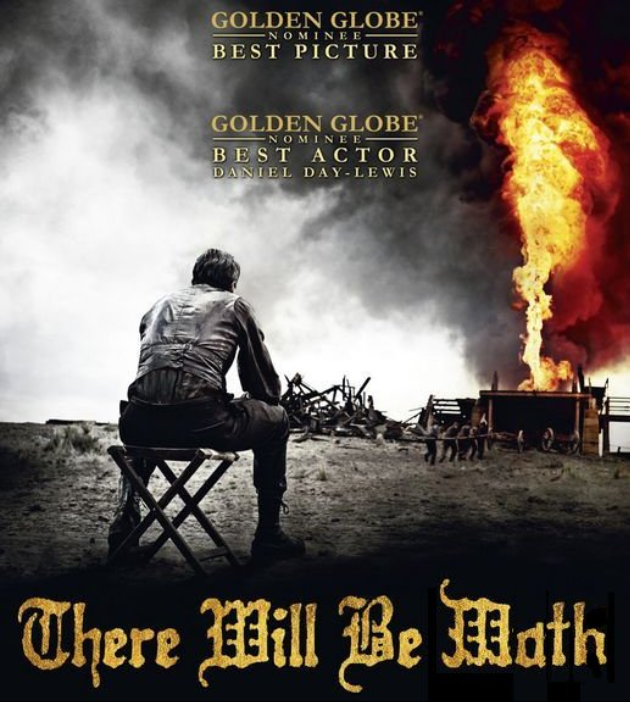
\includegraphics[width=.5\textwidth]{therewillbemath.png}
}

\end{frame}

\begin{frame}
\frametitle{Why do we care about probability and statistics?}

Recall, \blue{statistics} is the analysis and interpretation of data.

\vsp
In \red{machine learning}, we attempt to generalize from one ``training''
data set to general ``rules'' that can be applied to ``test'' data.

\vsp
\onslide<2->{
{\Large How is machine learning \emph{different} from statistics?}
}

\bee
\i<3-> Stats cares about the \blue{model}, we care about \red{predictions}
\i<4-> Stats cares about \blue{model fit}, we care about \red{generalization}
\i<5-> Stats tries to \blue{explain the world}, we try to \red{predict the future}
\ene

\onslide<6->{
\parbox{.4\textwidth}{
\Large \green{It all started with a lady drinking tea\dots}
}\parbox{.3\textwidth}{
\begin{center}
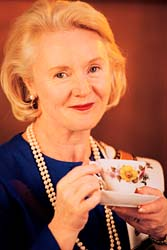
\includegraphics[height=.3\textheight]{ladydrinkingtea.jpg}
\end{center}
}\parbox{.3\textwidth}{
\begin{center}
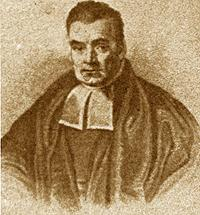
\includegraphics[width=.3\textheight]{Bayes.jpg}
\end{center}
}
}
\end{frame}

\begin{frame}
\frametitle{History of ML?}

\bei
\i Initial attempts at object recognition \citeit{Rosenblatt, 1958}
\i Learning to play checker \citeit{Samuel, 1959, 1963}
\i Rosenblatt can't learn XOR \citeit{Minsky \& Pappert, 1969}
\i Symbolic learning, spectroscopy \citeit{Winston, 1975; Buchanan 1971}
\i Backpropagation for neural nets \citeit{Werbos, 1974; Rummelhart, 1986}
\i PAC model of learning theory \citeit{Valiant, 1984}
\i Optimization enters machine learning \citeit{Bennett \& Mangasarian, 1993}
\i Kernel methods for non-linearity \citeit{Cortes \& Vapnik, 1995}
\i Machine learning behind day-to-day tasks \citeit{2005ish}
\i Machine learning takes over the world \citeit{2010ish}
\i Neural networks and the biggest come-back ever \citeit{2013ish}
\eni
\end{frame}


\end{document}


